Voici le document corrigé :

• la colonne « date » des expériences a une largeur fixe (3 cm) pour qu’elle n’empiète plus sur la marge droite ;  
• tous les blocs ou puces restés vides ont été supprimés (2ᵉ expérience, 2ᵉ formation, 2ᵉ certification, ligne « Website »).

```latex
\documentclass{article}

\usepackage{times}
\usepackage{geometry}
\geometry{a4paper,left=0.6cm,right=0.7cm,top=2cm,bottom=1cm,columnsep=0.8cm}
\usepackage{fontawesome}
\usepackage[hidelinks]{hyperref}
\usepackage{multicol}
\usepackage{tikz}
\usepackage{hyphsubst}
\usepackage{moresize}
\usepackage{hyphenat}
\usepackage{tabularx}          % <-- pour la colonne date
\usepackage{xcolor}
\usepackage{enumitem}

\newcolumntype{Y}{>{\RaggedRight\arraybackslash}X}
\newcolumntype{R}{>{\raggedleft\arraybackslash}p{3cm}} % <-- largeur fixe pour la date

\setlist[itemize]{itemsep=1pt,leftmargin=*,topsep=-10pt}

\definecolor{maincolor}{HTML}{f0fafc}
\definecolor{seccolor}{HTML}{ffffff}
\definecolor{gray}{HTML}{8c94a9}
\definecolor{sidetext}{HTML}{59cee5}

\usepackage[contents={}]{background}
\AddEverypageHook{\begin{tikzpicture}[remember picture,overlay]
  \node[inner sep=0pt,outer sep=0pt] at (current page.north west) [anchor=north west]{%
  \fcolorbox{maincolor}{maincolor}{%
\begin{minipage}[t][\paperheight][t]{0.3\paperwidth}
        \color{white}\hspace{0.08cm}
\end{minipage}}
\fcolorbox{seccolor}{seccolor}{
\begin{minipage}[t][\paperheight][t]{0.67\paperwidth}
        \color{black}\hspace{1cm}
\end{minipage}}
  };
\end{tikzpicture}}

\setlist[itemize]{itemsep=-2pt,topsep=0pt,leftmargin=1.08cm}
\renewcommand{\labelitemi}{\textcolor{sidetext}{\footnotesize$\bullet$}}

\setlength{\parindent}{0pt}
\usepackage{paracol}

\begin{document}
\pagestyle{empty}

\columnratio{0.3}
\begin{paracol}{2}

% ----------------- COLONNE GAUCHE -----------------
\color{sidetext}
\begin{center}
  \begin{tikzpicture}
    \clip (0,0) circle (1.5cm) node {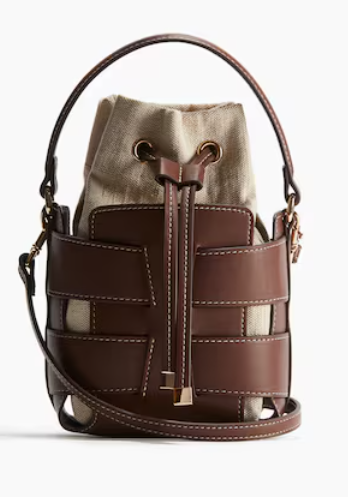
\includegraphics[width=3cm]{91408bcd4fc24aaeab45af38a2127443.png}};
  \end{tikzpicture}

  {\color{black}\LARGE\textbf{Pape Saliou FALL}}

  {\large Data Scientist}
\end{center}

{\color{gray}\rule{\linewidth}{0.4pt}}

\begin{tabular}{cl}
  \faPhone{} & \begin{tabular}{p{0.7\linewidth}}
     {\color{gray}Phone}\\ 0753481453
  \end{tabular} \\[6pt]

  \faLinkedin{} & \begin{tabular}{p{0.7\linewidth}}
    {\color{gray}LinkedIn}\\
    \href{https://www.linkedin.com/in/pape-saliou-fall-43154a211}{linkedin.com/in/pape-saliou-fall-43154a211}
  \end{tabular} \\[6pt]

  \faMapMarker{} & \begin{tabular}{p{0.7\linewidth}}
    {\color{gray}Address}\\ Paris, Île-de-France, France
  \end{tabular}
\end{tabular}

\vspace{.2cm}
{\color{gray}\rule{\linewidth}{0.4pt}}

{\color{black}Languages}

\begin{tabular}{cl}
  {\Large\faLanguage{}} &
  \begin{tabular}{l}
    French, English\\
    {\color{gray}Fluent}
  \end{tabular}
\end{tabular}

\vspace{10pt}
{\color{gray}\rule{\linewidth}{0.4pt}}

\vspace{.4cm}
{\color{black}Key Skills}

\begin{tabular}{ll}
  
\includegraphics[width=0.1\linewidth]{picon.png} & Python \\[8pt]
  
\includegraphics[width=0.1\linewidth]{picon.png} & R \\[8pt]
  
\includegraphics[width=0.1\linewidth]{picon.png} & SQL \\[8pt]
  
\includegraphics[width=0.1\linewidth]{picon.png} & Machine Learning \\[8pt]
  
\includegraphics[width=0.1\linewidth]{picon.png} & Deep Learning
\end{tabular}

% ----------------- COLONNE DROITE -----------------
\switchcolumn
\color{black}

\Large\textbf{Professional Summary}

Data Scientist with 3+ years of experience in building and deploying machine-learning models to solve business problems. Adept at transforming raw data into actionable insights using Python, SQL and cloud services. Passionate about continuous learning and delivering high-impact data solutions in agile environments.

\vspace{6pt}
\Large\textbf{Work Experience}

\colorbox{maincolor}{%
  \begin{minipage}{\linewidth}
    \begin{tabularx}{\linewidth}{@{}lX R@{}}
      
\includegraphics[width=0.05\linewidth]{picon.png} &
      Prepaya & {\footnotesize Jan 2022 -- Dec 2023}\\[-8pt]
      & {\color{sidetext}Data Scientist} &\\
      & {\small Paris, France} &
    \end{tabularx}
    \begin{itemize}
      \item Developed predictive models for customer churn using Python and scikit-learn.
    \end{itemize}
  \end{minipage}}

\vspace{1cm}
\Large\textbf{Education}

\begin{tabular}{@{}cp{0.7\linewidth}}
  
\includegraphics[width=0.05\linewidth]{picon.png} &
  \vspace{-12pt}{\color{sidetext}Master 2 – Data Science}\\[-6pt]
  & Sorbonne Université\\
  & 2012 – 2015
\end{tabular}

\vspace{0.5cm}
\Large\textbf{Certifications}

\begin{itemize}[leftmargin=12pt]
  \item ksLD — KSLQKBC (Jul-2024)
\end{itemize}

\end{paracol}
\end{document}
```

Les dates tiennent désormais dans la page et les emplacements vides n’apparaissent plus.